% ------------------------------------------------------------------------------------------------------------------------------------------------------
% The Pressure Poisson equation in FDS
% ------------------------------------------------------------------------------------------------------------------------------------------------------
\section{The Pressure Poisson equation in FDS}
\label{SEC_SCARC_poisson}

The pressure equation in FDS, an elliptic partial differential equation of second order which is commonly referred to as {\it Poisson equation}, reads as
\be 
  \nabla^2 \cH =-\dod{(\nabla \cdot {\bf u})}{t} - \nabla \cdot \bF\,.
  \label{EQ_SCARC_pressure}
\ee
Here, $\bu$ denotes the velocity field and $\bF$ the force term which includes the thermodynamic contributions from the previous time step such as radiation, combustion, pyrolysis, etc.  
The pressure term $\cH \equiv |\bu|^2/2 + \tp/\rho$ incorporates the density $\rho$ as well as the perturbation pressure $\tp$ by which the fluid motion is driven. The numerical solution of Equation (\ref{EQ_SCARC_pressure}) requires the specification of appropriate boundary conditions. Detailed information about its mathematical derivation and the possible types of boundary conditions can be found in the FDS Technical Reference Guide~\cite{McGrattan:2018:TG}.

The numerical time-stepping scheme in FDS, an {\it explicit second-order predictor/corrector scheme}, requires the solution of Equation (\ref{EQ_SCARC_pressure}) at least twice per time step which in total requires a considerable part of the overall computing time.
Because of its strong interaction with the calculation of all other thermodynamic quantities, the solution of the pressure equation is an essential step in the entire solution process and must be treated as efficiently and accurately as possible.

Due to the explicit character of the time-stepping scheme, FDS basically possesses a very high potential for parallelization.
While performing a new time step, each sub-mesh must only access values from the previous time step which have already been computed before. Typically only local data exchanges between neighboring sub-meshes are required which can be accessed with high computational efficiency on modern parallel architectures. 
%Of course, it would be highly preferable if the solution of the Poisson equation could also be done in a similar local way. How well this will finally be possible is analysed below.




% ------------------------------------------------------------------------------------------------------------------------------------------------------
% Discretization of the Poisson equation
% ------------------------------------------------------------------------------------------------------------------------------------------------------
\subsection{Discretization by finite differences}
\label{SEC_SCARC_discretization_poisson}

The first step towards a numerical solution of Equation (\ref{EQ_SCARC_pressure}) is to superimpose the computational domain $\Omega$ with a corresponding grid in whose cells the respective values of the analytical solution are determined only approximately. 
Thereby, based on default subdivision into structured rectangular cells within FDS,
the spatial derivative of $\hp$ in Equation (\ref{EQ_SCARC_pressure}) is replaced by a 
{\it central difference quotient} which is evaluated in the centers of the individual grid cells.  In case of equidistant grid size $h$, %=\dx=\dy=\dz$, 
Figure~(\ref{FIG_SCARC_five_point_stencil}) sketches the underlying well-known {\it 7-point stencil} in 3D which approximates the second derivative cell by cell, as well as its 2D counterpart.
%
The final discretized version of the Poisson equation looks like
\small
\begin{align}
\frac{\hp_{i+1,jk}-2\hp_{ijk}+\hp_{i-1,jk}}{\dx^2} +
\frac{\hp_{i,j+1,k}-2\hp_{ijk}+\hp_{i,j-1,k}}{\dy^2} +
\frac{\hp_{ij,k+1}-2\hp_{ijk}+\hp_{ij,k-1}}{\dz^2} \notag \\ =
    -\frac{F_{\x,ijk} - F_{\x,i-1,jk}}{\dx}
    -\frac{F_{\y,ijk} - F_{\y,i,j-1,k}}{\dy}
    -\frac{F_{\z,ijk} - F_{\z,ij,k-1}}{\dz} - \frac{\delta}{\delta t}(\nabla\!\cdot \bu)_{ijk}\,.
\label{EQ_SCARC_discrete_poisson}
\end{align}
\normalsize
The {\it finite difference} approximation (\ref{EQ_SCARC_discrete_poisson})
of $\hp$ turns out to be of second-order accuracy, that is, the error between the analytical and numerical solution is proportional to the 2th power of the grid width.
Note, that different discretizations for the time derivative of the velocity divergence are used in the predictor and corrector parts of the time stepping scheme, see again the FDS Technical Reference Guide\cite{McGrattan:2018:TG} for more details. 

\begin{figure}[htb]
\begin{center}
%
\begin{minipage}[htb]{0.6\textwidth}
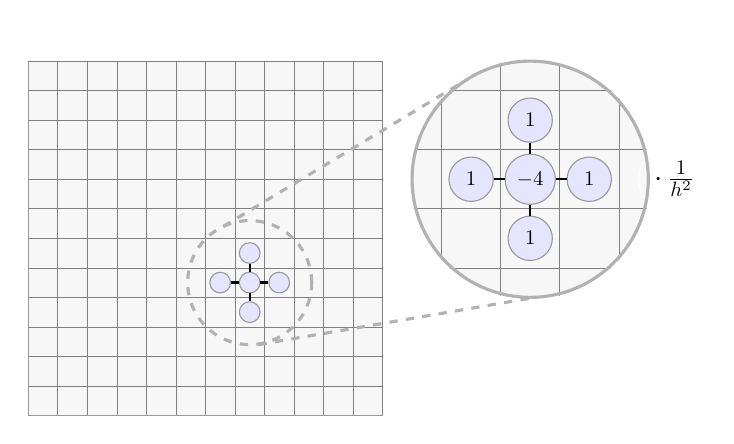
\begin{tikzpicture}
[
 scale=0.75,
 every node/.style ={scale=0.75},
 inner sep=1mm,
 %scale=1.0,
 L3/.style={circle, draw=black!0,  minimum size=3.5mm},
 L2/.style={circle, draw=black!40, fill=blue!10, thin, minimum size=3.5mm},
 L2A/.style={circle, draw=black!40, fill=blue!10, thin, minimum size=7.5mm},
 L1/.style={rectangle, draw=black!40, fill=black!03,   thin, minimum size=6cm},
 inner sep=0.6mm,
 X/.style={circle, draw=black!100, fill=black!03, thin, minimum size=4cm},
 X2/.style={circle,draw=white, line width=4mm, minimum size=4.6cm}
 ],
 %
\node [X]  at ( 10.5, 6)  {};
\draw[step=1cm,gray,very thin] (8.5,4.5) -- (12.5,4.5);
\draw[step=1cm,gray,very thin] (8.5,5.5) -- (12.5,5.5);
\draw[step=1cm,gray,very thin] (8.5,6.5) -- (12.5,6.5);
\draw[step=1cm,gray,very thin] (8.5,7.5) -- (12.5,7.5);
\draw[step=1cm,gray,very thin] (9,4) -- (9,8);
\draw[step=1cm,gray,very thin] (10,4) -- (10,8);
\draw[step=1cm,gray,very thin] (11,4) -- (11,8);
\draw[step=1cm,gray,very thin] (12,4) -- (12,8);
%
\node [X2] at (10.5, 6) {};
%
\draw (10.5, 6) circle  (2cm);
\node [L2A]  (M2)   at ( 10.5, 6)  {\normalsize $\;-4\;$};
\node [L2A]  (S2)    at ( 10.5, 5)  {\normalsize $1$};
\node [L2A]  (W2)   at ( 9.5, 6)  {\normalsize $1$};
\node [L2A]  (E2)    at ( 11.5, 6)  {\normalsize $1$};
\node [L2A]  (N2)    at ( 10.5, 7)  {\normalsize $1$};
\node [L3]    at ( 12.9, 6)  {\Large \,$\cdot \,\frac{1}{h^2}$};
%
\draw [thick]  (M2.south)  -- (S2.north) ;
\draw [thick]  (M2.west) -- (W2.east) ;
\draw [thick]  (M2.north) -- (N2.south) ;
\draw [thick]  (M2.east) -- (E2.west) ;
%
\node [L1]    at ( 5, 5)  {};
\draw[step=0.5cm,gray,very thin] (2,2) grid (8,8);
%\draw[step=8cm,thick] (2,2) grid (6,6);

%
\node [L2]  (M)   at ( 5.75, 4.25)  {};
\node [L2]  (S)    at ( 5.75, 3.75)  {};
\node [L2]  (W)   at ( 5.25, 4.25)  {};
\node [L2]  (E)    at ( 6.25, 4.25)  {};
\node [L2]  (N)    at ( 5.75, 4.75)  {};
%
\draw [line width=.4mm, draw=black!30,dashed] (5.75,4.25) circle (1.05cm);
\draw [line width=.4mm, draw=black!30] (10.5,6) circle (2cm);
\draw [line width=.4mm, draw=black!30,dashed] (5.3,5.2) -- (9.45,7.7);
\draw [line width=.4mm, draw=black!30,dashed] (5.9,3.2) -- (10.53,3.99);

%
\draw [thick]  (M.south)  -- (S.north) ;
\draw [thick]  (M.west) -- (W.east) ;
\draw [thick]  (M.north) -- (N.south) ;
\draw [thick]  (M.east) -- (E.west) ;

%
\end{tikzpicture}

\end{minipage}
\hspace{-1.5cm}
\begin{minipage}[htb]{0.25\textwidth}


%\def\myarray{{"blue!05", "blue!20", "blue!40"}}
\def\myarray{{"blue!10", "blue!10", "blue!10"}}
\def\xk{0.3}
\def\yk{0.2}
\def\xs{0.9}
\def\ys{0.8}
\def\xl{1.5}
\def\yl{1.5}

 \def\dia{0.5em}
 \def\dist{1.5}
 \def\xnull{0.3}
 \def\ynull{0.2}

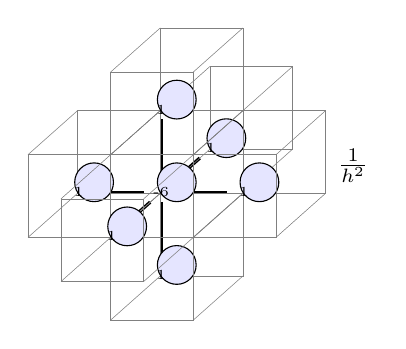
\begin{tikzpicture}[scale=0.7]
 \node  (M) at (\xnull,\ynull) {\makebox[\dia]{}};

 \node  (T) at (\xnull,\ynull+\dist) {\makebox[\dia]{}};
 \draw[very thick] (M) -- (T);

 \node (Bo) at (\xnull,\ynull-\dist) {\makebox[\dia]{}};
 \draw[very thick] (M) -- (Bo);

 \node (L) at (\xnull-\dist,\ynull) {\makebox[\dia]{}};
 \draw[very thick] (M) -- (L);

 \node  (R) at (\xnull+\dist,\ynull) {\makebox[\dia]{}};
 \draw[very thick] (M) -- (R);

 \node  (F) at (\xnull-\xs,\ynull-\ys) {\makebox[\dia]{}};
 \draw[very thick] (M) -- (F);

 \node  (Ba) at (\xnull+\xs,\ynull+\ys) {\makebox[\dia]{}};
 \draw[very thick] (M) -- (Ba);

\ifnum1=1 % auf =0 setzen, um das Gitter auszublenden
\foreach \z in {-1, 0,1} {
  \foreach \x in {-1, 0,1} {
    \pgfmathmultiply{\z}{\xs}
    \let\xshift\pgfmathresult
    \pgfmathmultiply{\x}{\xl}
    \pgfmathsubtract{\pgfmathresult}{\xshift}
    \let\xnull\pgfmathresult
    \foreach \y in {-1, 0,1} {
      \pgfmathparse{(\x==0 && \y==0) || (\x==0 && \z==0) || (\z==0 && \y==0) ?int(1):int(0)}
      \ifnum\pgfmathresult>0\relax
      \pgfmathmultiply{\z}{\ys}
      \let\yshift\pgfmathresult
      \pgfmathmultiply{\y}{\yl}
      \pgfmathsubtract{\pgfmathresult}{\yshift}
      \let\ynull\pgfmathresult
      \draw[very thin,gray] (\xnull,\ynull) -- (\xnull,\ynull+\yl) -- (\xnull+\xl,\ynull+\yl) -- (\xnull+\xl,\ynull) -- cycle;
      \draw[very thin,gray] (\xnull-\xs,\ynull-\ys) -- (\xnull,\ynull);
      \draw[very thin,gray] (\xnull+\xl-\xs,\ynull-\ys) -- (\xnull+\xl,\ynull);
      \draw[very thin,gray] (\xnull-\xs,\ynull+\yl-\ys) -- (\xnull,\ynull+\yl);
%        \pgfmathparse{\myarray[\z+1]}
%        \draw[fill=\pgfmathresult] (\xk+\xnull,\yk+\ynull) circle (1em);
      \draw[fill=blue!10] (\xk+\xnull,\yk+\ynull) circle (1em);
%      \node [circle,draw,fill=blue!10]  at (\xk+\xnull,\yk+\ynull)  {\makebox[\dia]{}};
      \draw[very thin,gray] (\xnull+\xl-\xs,\ynull+\yl-\ys) -- (\xnull+\xl,\ynull+\yl);
      \draw[very thin,gray] (\xnull-\xs,\ynull-\ys) -- (\xnull-\xs,\ynull-\ys+\yl) -- (\xnull-\xs+\xl,\ynull-\ys+\yl) -- (\xnull-\xs+\xl,\ynull-\ys) -- cycle;
      \fi
    }
  }
}
\fi

 \node at (M)  {\tiny -6};
 \node at (T)  {\tiny 1};
 \node at (Bo) {\tiny 1};
 \node at (L) {\tiny 1};
 \node at (R) {\tiny 1};
 \node at (F) {\tiny 1};
 \node at (Ba) {\tiny 1};

 \node at (3.5,0.5) { $ \frac{1}{h^2} $ };
\end{tikzpicture}

\vspace{-0.6cm}
\end{minipage}
%
\caption{Central difference quotients: (Left) 5-point stencil in 2D. (Right) 7-point stencil in 3D.}
\label{FIG_SCARC_five_point_stencil}
\end{center}
\end{figure}

Typically, this discretization process leads to a huge system of equations, which has to be solved efficiently by means of a suitable numerical solver.
The growing complexity of contemporary applications thereby increasingly requires the use of high performance computers and corresponding discretizations, which are suitable for parallel application.

\subsubsection{Global versus local discretization}
\label{SEC_SCARC_poisson_global_vs_local}
In order to describe the underlying discretization processes and the basic operation principles of the various Poisson solvers available in FDS,
Figure \ref{FIG_SCARC_basic_pipe_geometry} introduces a small pipe-shaped geometry in 2D. This simple demonstration case is used repeatedly throughout the entire documentation and is also the basis for later test calculations.
\begin{figure}[ht]
\begin{center}
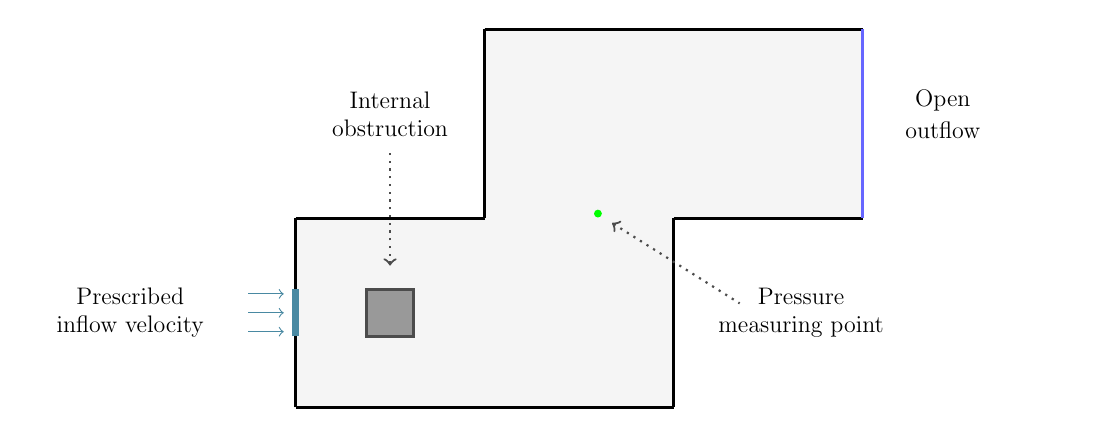
\begin{tikzpicture}
[
scale=0.6,
every node/.style ={scale=0.6},
Background/.style={rectangle,draw=black!04,fill=black!04, thin, minimum size = 4 cm},
Obstruction/.style={rectangle,draw=black!70,fill=black!40, very thick, minimum size=1cm},
Finegrid/.style={step=0.5cm,gray,very thin},
Thickline/.style={-,draw=black!100,fill=black!02, very thick},
Thinline/.style={draw=black!100,fill=black!02, very thin},
Inflow/.style={-,draw={rgb,255:red,73;green,137;blue,162},line width=0.8mm},
Inarrow/.style={->,draw={rgb,255:red,73;green,137;blue,162},thin},
Outflow/.style={-,draw=blue!60,very thick},
Ball/.style={circle, draw=black!40, fill=red!20, thin, minimum size=3.5mm},
Circle/.style={circle,draw=black!40,fill=black!06,thin,minimum size=35.5mm},
Rectangle/.style={rectangle,draw=black!10,fill=white,inner xsep=0pt, inner ysep=0pt,},
Box/.style = {very thin, rectangle, inner xsep=10pt, inner ysep=10pt,},
%Device/.style={fill={rgb,255:red,192;green,58;blue,10}, draw={rgb,255:red,192;green,58;blue,10}},
Device/.style={fill=green, draw=green},
Arrow/.style={thick, dotted, draw=black!70}
]

\node[Background] at (2,2) {};
\node[Background] at (6,2) {};
\node[Background] at (6,6) {};
\node[Background] at (10,6) {};

\node[Obstruction] at (2,2) {};

\draw[Thickline] (0,0)--(8,0);
\draw[Thickline] (4,8)--(12,8);
\draw[Thickline] (0,4)--(4,4);
\draw[Thickline] (8,4)--(12,4);

\draw[Thickline] (0,0)--(0,4);
\draw[Thickline] (4,8)--(12,8);
\draw[Thickline] (4,4)--(4,8);
\draw[Thickline] (8,0)--(8,4);
\draw[Thickline] (12,4)--(12,8);

\draw[Inflow]   (0,1.5)--(0,2.5);
\draw[Inarrow]  (-1,1.6)--(-0.25,1.6);
\draw[Inarrow]  (-1,2.0)--(-0.25,2.0);
\draw[Inarrow]  (-1,2.4)--(-0.25,2.4);
\draw[Outflow]  (12,4)--(12,8);

\draw[Device] (6.4,4.1) circle (2pt);
\draw [<-, Arrow] (6.7,3.9) -- (9.4,2.2);
\draw [<-, Arrow] (2.0,3.0) -- (2.0,5.4);
\node [Box] (Box) at (-3.5,2.0)  {\begin{minipage}{0.3\textwidth}\centering{\Large Prescribed\\[0.8ex] inflow velocity}\end{minipage}};
\node [Box] (Box) at (13.7,6.2){\begin{minipage}{0.4\textwidth}\centering{\Large Open \\[0.8ex] outflow}\end{minipage}};
\node [Box] (Box) at (2.0,6.2)  {\begin{minipage}{0.4\textwidth}\centering{\Large Internal \\[0.8ex] obstruction}\end{minipage}};
\node [Box] (Box) at (10.7,2.0){\begin{minipage}{0.4\textwidth}\centering{\Large Pressure  \\[0.8ex] measuring point}\end{minipage}};
\end{tikzpicture}


\end{center}
\caption[Pipe-shaped geometry in 2D]{Pipe-shaped example geometry in 2D with a small internal obstruction,
a predefined inflow from the left, a pressure measuring point for the pressure and an open outflow on the right.}
\label{FIG_SCARC_basic_pipe_geometry}
\end{figure}

If the whole pipe geometry is discretized in one piece, one global system of equations is obtained,
\be 
  Ax = b\,, 
  \label{EQ_SCARC_single_system}
\ee
whereby $n$ denotes the number of total grid cells, 
$x, \,b\in\mathbb{R}^n$ the corresponding solution and right hand side vectors and $A \in \mathbb{R}^{n \times n}$ the overall Poisson matrix. 

However, since FDS is based on partitions of the computational domain into $M$ rectilinear sub-meshes $\Omega_i$ with regular local grids each, every sub-mesh holds its own system of equations 
\be 
   A_i x_i = b_i\,, \qquad i=1, \ldots, M, 
  \label{EQ_SCARC_multi_system}
\ee
with corresponding local numbers of grid cells $n_i$,  local solution and right hand side vectors $x_i, b_i \in \mathbb{R}^{n_i}$ and locally defined Poisson matrices $A_i \in \mathbb{R}^{n_i \times n_i}$. 
A more formal definition of these quantities will be given in Section (\ref{SEC_SCARC_block_precon}).
The resulting global and local discretization processes are illustrated in Figure \ref{FIG_SCARC_global_vs_local_discretization}.



\begin{figure}[ht]
\begin{center}
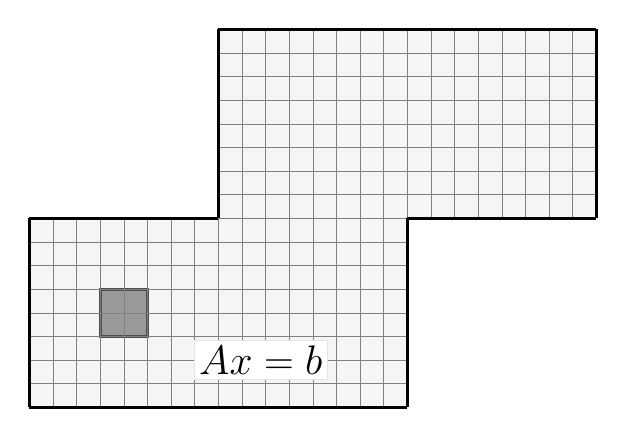
\begin{tikzpicture}
[
scale=0.6,
every node/.style ={scale=0.6},
Background/.style={rectangle,draw=black!04,fill=black!04, thin, minimum size = 4 cm},
Obstruction/.style={rectangle,draw=black!70,fill=black!40, very thick, minimum size=1cm},
Finegrid/.style={step=0.5cm,gray,very thin},
Thickline/.style={-,draw=black!100,fill=black!02, very thick},
Thinline/.style={draw=black!100,fill=black!02, very thin},
Ball/.style={circle, draw=black!40, fill=red!20, thin, minimum size=3.5mm},
Circle/.style={circle,draw=black!40,fill=black!06,thin,minimum size=35.5mm},
%Rectangle/.style={rectangle,color=blue, inner xsep=7pt, inner ysep=7pt,},
%Rectangle/.style={rectangle,color={rgb,255:red,192;green,58;blue,10}, inner xsep=7pt, inner ysep=7pt,},
Rectangle/.style={rectangle,draw=black!10,fill=white,inner xsep=3pt, inner ysep=3pt,},
box/.style = {very thin, rectangle, inner xsep=10pt, inner ysep=10pt,},
]

\node[Background] at (2,2) {};
\node[Background] at (6,2) {};
\node[Background] at (6,6) {};
\node[Background] at (10,6) {};

\node[Obstruction] at (2,2) {};

\draw[Finegrid] (0,0) grid (8,4);
\draw[Finegrid] (4,4) grid (12,8);

\draw[Thickline] (0,0)--(8,0);
\draw[Thickline] (4,8)--(12,8);
\draw[Thickline] (0,4)--(4,4);
\draw[Thickline] (8,4)--(12,4);

\draw[Thickline] (0,0)--(0,4);
\draw[Thickline] (4,8)--(12,8);
\draw[Thickline] (4,4)--(4,8);
\draw[Thickline] (8,0)--(8,4);
\draw[Thickline] (12,4)--(12,8);

\vspace{1cm}

\node[Rectangle] at (4.9,1.0) {\Huge $Ax=b$};

\end{tikzpicture}
\quad\quad
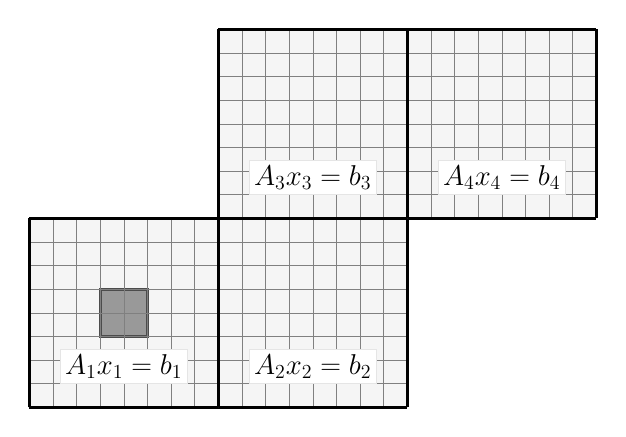
\begin{tikzpicture}
[
scale=0.6,
every node/.style ={scale=0.6},
Background/.style={rectangle,draw=black!04,fill=black!04, thin, minimum size = 4 cm},
Obstruction/.style={rectangle,draw=black!70,fill=black!40, very thick, minimum size=1cm},
Finegrid/.style={step=0.5cm,gray,very thin},
Thickline/.style={-,draw=black!100,fill=black!02, very thick},
Thinline/.style={draw=black!100,fill=black!02, very thin},
Ball/.style={circle, draw=black!40, fill=red!20, thin, minimum size=3.5mm},
Circle/.style={circle,draw=black!40,fill=black!06,thin,minimum size=35.5mm},
%Rectangle/.style={rectangle,color=blue, inner xsep=7pt, inner ysep=7pt,},
%Rectangle/.style={rectangle,color={rgb,255:red,192;green,58;blue,10}, inner xsep=7pt, inner ysep=7pt,},
Rectangle/.style={rectangle,draw=black!10,fill=white,inner xsep=3pt, inner ysep=3pt,},
box/.style = {very thin, rectangle, inner xsep=10pt, inner ysep=10pt,},
]

\node[Background] at (2,2) {};
\node[Background] at (6,2) {};
\node[Background] at (6,6) {};
\node[Background] at (10,6) {};

\node[Obstruction] at (2,2) {};

\draw[Finegrid] (0,0) grid (8,4);
\draw[Finegrid] (4,4) grid (12,8);

\draw[Thickline] (0,0)--(8,0);
\draw[Thickline] (4,8)--(12,8);
\draw[Thickline] (0,4)--(4,4);
\draw[Thickline] (8,4)--(12,4);

\draw[Thickline] (0,0)--(0,4);
\draw[Thickline] (4,8)--(12,8);
\draw[Thickline] (4,4)--(4,8);
\draw[Thickline] (8,0)--(8,4);
\draw[Thickline] (12,4)--(12,8);

\draw[Thickline] (4,0)--(4,4);
\draw[Thickline] (4,4)--(8,4);
\draw[Thickline] (8,4)--(8,8);

\node[Rectangle] at ( 2,0.86) {\LARGE $\boldsymbol{A_1x_1=b_1}$};
\node[Rectangle] at ( 6,0.86) {\LARGE $\boldsymbol{A_2x_2=b_2}$};
\node[Rectangle] at ( 6,4.86) {\LARGE $\boldsymbol{A_3x_3=b_3}$};
\node[Rectangle] at (10,4.86) {\LARGE $\boldsymbol{A_4x_4=b_4}$ };

\vspace{4cm}

%\node[Rectangle] at (16,2) {\textcolor{hhpred} {\Huge $ x \,\overset{ \mbox{\raisebox{1mm}{?}}}{=}\, \summv x_i$}};

\end{tikzpicture}

%\includegraphics[width=0.4\textwidth]{pictures/single_system_of_equations.png}\quad\quad
%\includegraphics[width=0.4\textwidth]{pictures/multiple_systems_of_equations.png}
\end{center}
\caption[Global discretization versus collection of local discretizations]{Different discretization types for the Poisson problem on the 2D-pipe with 4 meshes: (Left) Global discretization with one globally defined system of equations $Ax=b$. (Right) Local discretization with four locally defined systems of equations $A_i x_i=b_i$.}
\label{FIG_SCARC_global_vs_local_discretization}
\end{figure}
Note that a global discretization can also be achieved in a multi-mesh context, i.e. in a {\it data-parallel} sense. 
For this purpose, each mesh stores the respective parts of the solution and right-side vector as well as the global matrix, 
%that is, $A_i\$ is  the restriction of the global matrix $A$ to the sub-mesh $\Omega_i$, 
informally spoken ``$\,A_i \equiv \restrict{A}{\Omega_i}$''.
By means of suitable data exchanges between adjacent meshes the individual matrix-vector operations are then performed 
in exactly the same way as would also be the case with an actual global execution.

With regard to parallelization the use of local discretizations seems to be the more natural approach. 
Thus, the crucial question is, if there are appropriate solutions strategies for the local discretization type 
such that the obtained collection of mesh-wise solutions is comparably accurate as the overall solution for the corresponding global discretization, i.e. $\sum_{i=1, \ldots, M}\, x_i \sim x$. 
This question will be addressed with respect to the various Poisson solvers below.


% ------------------------------------------------------------------------------------------------------------------------------------------------------
% Structured versus unstructured Discretization
% ------------------------------------------------------------------------------------------------------------------------------------------------------
\subsubsection{Structured versus unstructured discretization}
\label{SEC_SCARC_discretization_types}

For the discretization of the single meshes two different strategies can be applied in FDS. They essentially differ in how they treat cells internal to solid objects within the domain and their neighboring gas-phase cells. Both types have their advantages and disadvantages and significantly determine which solution strategy can be applied at all. 
%In FDS, both types are available in combination with appropriate solution strategies and 
%will later be compared by means of several test series.
%
To illustrate the differences between the two, Figure \ref{FIG_SCARC_structured_vs_unstructured_discretization} illustrates the respective matrix stencils and grid numberings. Therein, both plots are related to
the lower left mesh of the 2D pipe geometry containing the internal obstruction as can be seen in the right plot of \ref{FIG_SCARC_global_vs_local_discretization} again for the case of local discretization.
%\begin{itemize}
%\item 
\paragraph{Structured discretization:}  This type explicitly includes both, gas-phase and solid cells,
and is the default type in FDS. Cells internal to solid obstructions are masked as blocked cells. But the same matrix stencil is applied all over the domain, regardless whether the underlying cell is a gas-phase or a solid cell. Without any exception all grid cells are incorporated into the resulting discretization matrix which therefore takes a very regular shape. As a major advantage this strategy allows the use of highly tuned solvers developed specifically for regular grids which can be performed with enormous computational efficiency. But, there is no way to describe the correct boundary conditions along internal objects:
While the no-flux boundary condition is exact at external boundaries, it is not possible to prescribe the required homogeneous no-flux condition at internal boundaries directly. Erroneously, 
the velocity field may contain non-zero contributions towards internal solids
associated with a corresponding loss of accuracy which represents the greatest disadvantage of this strategy. By using appropriate corrective actions, this effect can be remedied as is also done in FDS and will be described below.

%\item 
\paragraph{Unstructured discretization:} This type only incorporates the gas-phase cells while it omits all solid cells from the system of equations. This strategy is the only way to completely get rid of the undesirable penetration errors. On gas-phase cells which are directly adjacent to the surface of an obstruction the homogeneous no-flux Neumann condition is explicitly specified and included into the matrix. Thus, the greatest advantage of this approach is that it offers more accuracy because the correct boundary information along  internal obstructions can now be included into the system. But, in contrast to the structured case this strategy requires the usage of individual matrix stencils for the different grid cells depending on their location with respect to obstructions. While the resulting unstructured matrix has less entries than the corresponding structured one, it no longer has a regular shape and makes higher demands on the robustness of the solver, which may comprehensively limit the achievable efficiency and is the main disadvantage of this approach. 
%\end{itemize}

\vspace{0.5cm}
Furthermore, Figure \ref{FIG_structured_vs_unstructured_spy} opposes the sparsity patterns of the resulting Poisson matrices to each other. As can be seen clearly, both discretization types lead to sparse matrices which basically have only very less non-zero elements. Based on the underlying stencils the non-zeros are restricted to only a few diagonal bands (5 in 2D, 7 in 3D),
which is extremely less compared to the number of possible entries.
For mesh 1 in the local discretization of the 2D-pipe, consisting of $n_1$ cells in total, this amounts to only about $5 n_1$ entries compared to the possible number of entries $n_1^2$. 
Note, that these are the values which have to be stored on the computing system and therefore significantly determine the memory requirements for the solver in use.

However, it also becomes apparent that the structured discretization results in a highly regular matrix with a constantly repeating pattern, while the unstructured discretization shows irregularities associated with the different treatment of the internal obstruction as indicated with the red circle in the right plot. 
For a simple obstruction like the one considered here, the differences are not big, but the situation is completely different for more realistic applications with complex geometric details. In any case, the mentioned optimized solvers for regular grids can no longer be applied in the unstructured case and more generally applicable solvers must be used.


Note, that the unstructured discretization even leads to less matrix entries since the obstruction wasn't included in the discretization process. But this supposed advantage typically does not carry weight due to the more complex matrix structure and the increased demands on a respective solver.


\begin{figure}[H]
\begin{center}
\begin{minipage}[b]{0.475\textwidth}
\centering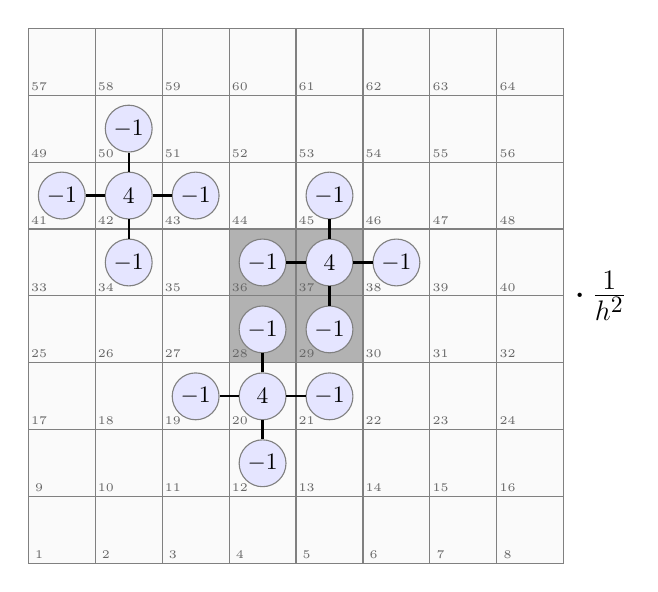
\begin{tikzpicture}
[
 scale=0.85,
 every node/.style ={scale=0.85},
 inner sep=0.5mm,
 BLUECIRC/.style={circle, draw=black!50, fill=blue!10, thin, minimum size=7.0mm},
 REDCIRC/.style={circle, draw=black!50, fill=red!10, thin, minimum size=7.0mm},
 OBST/.style={rectangle, draw=black!50, fill=black!30, thin, minimum size=10mm},
 CELL/.style={rectangle, draw=black!50, fill=black!02,   thin, minimum size=10mm},
 ],
%
\foreach \y in {1,2,3,4,5,6,7,8}
   \foreach \x in {1,2,3,4,5,6,7,8}
      {
        \node [CELL]    at ( \x, \y)  {};
       }
\foreach \y in {4,5}
   \foreach \x in {4,5} { \node [OBST]    at ( \x, \y)  {}; }
%
\node  at (9.0,4.5)  {\LARGE \,$\cdot \,\frac{1}{h^2}$};       
%
\node [BLUECIRC]  (XS)   at ( 4, 2)  {$-1$};
\node [BLUECIRC]  (XW)   at ( 3, 3)  {$-1$};
\node [BLUECIRC]  (XC)   at ( 4, 3)  {$4$};
\node [BLUECIRC]  (XN)   at ( 4, 4)  {$-1$};
\node [BLUECIRC]  (XE)   at ( 5, 3)  {$-1$};
%
\node [BLUECIRC]  (YS)   at ( 2, 5)  {$-1$};
\node [BLUECIRC]  (YW)   at ( 1, 6)  {$-1$};
\node [BLUECIRC]  (YC)   at ( 2, 6)  {$4$};
\node [BLUECIRC]  (YN)   at ( 2, 7)  {$-1$};
\node [BLUECIRC]  (YE)   at ( 3, 6)  {$-1$};
%
\node [BLUECIRC]  (ZS)   at ( 5, 4)  {$-1$};
\node [BLUECIRC]  (ZW)   at ( 4, 5)  {$-1$};
\node [BLUECIRC]  (ZC)   at ( 5, 5)  {$4$};
\node [BLUECIRC]  (ZN)   at ( 5, 6)  {$-1$};
\node [BLUECIRC]  (ZE)   at ( 6, 5)  {$-1$};
%
\draw [thick]  (XC.south)  -- (XS.north) ;
\draw [thick]  (XC.west)   -- (XW.east) ;
\draw [thick]  (XC.north)  -- (XN.south) ;
\draw [thick]  (XC.east)  -- (XE.west) ;
%
\draw [thick]  (YC.south)  -- (YS.north) ;
\draw [thick]  (YC.west)   -- (YW.east) ;
\draw [thick]  (YC.north)  -- (YN.south) ;
\draw [thick]  (YC.east)  -- (YE.west) ;
%
\draw [thick]  (ZC.south)  -- (ZS.north) ;
\draw [thick]  (ZC.west)   -- (ZW.east) ;
\draw [thick]  (ZC.north)  -- (ZN.south) ;
\draw [thick]  (ZC.east)  -- (ZE.west) ;
%
\foreach \y in {0,1,2,3,4,5,6,7} {
  \pgfmathsetmacro{\ypos}{(\y+0.63)}
  \foreach \x in {0,1,2,3,4,5,6,7} {
    \pgfmathsetmacro{\xpos}{(\x+0.66)}
    \pgfmathsetmacro{\num}{int(8*\y+\x+1)}
    \draw[color=black!60]   node at (\xpos,\ypos) {\tiny \num};
  }
}
%
\end{tikzpicture}


\end{minipage}
\hspace{5mm}
\begin{minipage}[b]{0.475\textwidth}
\centering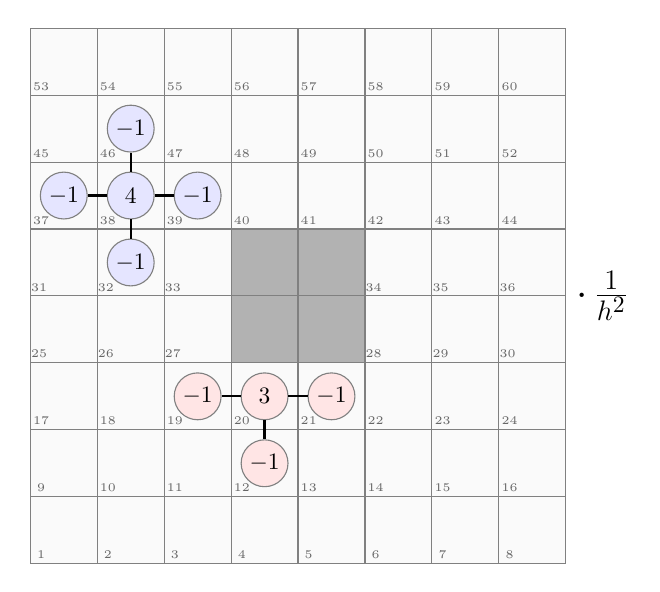
\begin{tikzpicture}
[
 scale=0.85,
 every node/.style ={scale=0.85},
 inner sep=0.5mm,
 BLUECIRC/.style={circle, draw=black!50, fill=blue!10,  thin, minimum size=7.0mm},
 REDCIRC/.style={circle, draw=black!50, fill=red!10, thin, minimum size=7.0mm},
 OBST/.style={rectangle, draw=black!50, fill=black!30, thin, minimum size=10mm},
 CELL/.style={rectangle, draw=black!50, fill=black!02,   thin, minimum size=10mm},
 ],
%      
\foreach \y in {1,2,3,4,5,6,7,8}
   \foreach \x in {1,2,3,4,5,6,7,8}
      {
        \node [CELL]    at ( \x, \y)  {};
       }
\foreach \y in {4,5}
   \foreach \x in {4,5} { \node [OBST]    at ( \x, \y)  {}; }
%
\node  at (9.0,4.5)  {\LARGE \,$\cdot \,\frac{1}{h^2}$};       
%
\node [REDCIRC]  (XS)   at ( 4, 2)  {$-1$};
\node [REDCIRC]  (XW)   at ( 3, 3)  {$-1$};
\node [REDCIRC]  (XC)   at ( 4, 3)  {$3$};
\node [REDCIRC]  (XE)   at ( 5, 3)  {$-1$};
%
\node [BLUECIRC]  (YS)   at ( 2, 5)  {$-1$};
\node [BLUECIRC]  (YW)   at ( 1, 6)  {$-1$};
\node [BLUECIRC]  (YC)   at ( 2, 6)  {$4$};
\node [BLUECIRC]  (YN)   at ( 2, 7)  {$-1$};
\node [BLUECIRC]  (YE)   at ( 3, 6)  {$-1$};
%
\draw [thick]  (XC.south) -- (XS.north) ;
\draw [thick]  (XC.west)  -- (XW.east) ;
\draw [thick]  (XC.east)  -- (XE.west) ;
%
\draw [thick]  (YC.south) -- (YS.north) ;
\draw [thick]  (YC.west)  -- (YW.east) ;
\draw [thick]  (YC.east)  -- (YE.west) ;
\draw [thick]  (YC.north) -- (YN.south) ;
%
\pgfmathsetmacro{\num}{int(0)}
\foreach \y in {0,1,2} {
  \pgfmathsetmacro{\ypos}{(\y+0.63)}
  \foreach \x in {0,1,2,3,4,5,6,7} {
    \pgfmathsetmacro{\xpos}{(\x+0.66)}
    \pgfmathsetmacro{\num}{int(8*\y+\x+1)}
    \draw[color=black!60]   node at (\xpos,\ypos) {\tiny \num};
  }
}
%
\draw[color=black!60]   node at (0.63,3.63) {\tiny 25};
\draw[color=black!60]   node at (1.63,3.63) {\tiny 26};
\draw[color=black!60]   node at (2.63,3.63) {\tiny 27};
\draw[color=black!60]   node at (5.63,3.63) {\tiny 28};
\draw[color=black!60]   node at (6.63,3.63) {\tiny 29};
\draw[color=black!60]   node at (7.63,3.63) {\tiny 30};
%
\draw[color=black!60]   node at (0.63,4.63) {\tiny 31};
\draw[color=black!60]   node at (1.63,4.63) {\tiny 32};
\draw[color=black!60]   node at (2.63,4.63) {\tiny 33};
\draw[color=black!60]   node at (5.63,4.63) {\tiny 34};
\draw[color=black!60]   node at (6.63,4.63) {\tiny 35};
\draw[color=black!60]   node at (7.63,4.63) {\tiny 36};
%
\foreach \y in {5,6,7} {
  \pgfmathsetmacro{\ypos}{(\y+0.63)}
  \foreach \x in {0,1,2,3,4,5,6,7} {
    \pgfmathsetmacro{\xpos}{(\x+0.66)}
    \pgfmathsetmacro{\num}{int(8*\y+\x-3)}
    \draw[color=black!60]   node at (\xpos,\ypos) {\tiny \num};
  }
}
%
\end{tikzpicture}

\end{minipage}
\end{center}
\caption[Structured versus unstructured discretization]{Matrix stencils and grid numberings for structured and unstructured discretizations:\\
(Left) The structured discretization uses the same matrix stencil everywhere, including cells internal to the solid obstruction. 
%The cell numbers are only determined by the grid dimensions in the different coordinate directions. 
Based on a lexicographic numbering the connectivity graph of the matrix is defined a-priori and and the resulting matrix takes a highly regular shape. \\
(Right) The unstructured discretization uses individual matrix stencils, excluding cells internal to the solid obstruction. There is no consecutive numbering anymore. Instead, an additional connectivity graph must be stored which specifies the neighbor relations between the single grid cells. For gas-phase cells adjacent to the obstruction the homogeneous boundary conditions are individually incorporated into the matrix which no longer has a regular shape.}
\label{FIG_SCARC_structured_vs_unstructured_discretization}
%\end{figure}
%\begin{figure}[ht]
\begin{center}
\begin{minipage}[b]{0.475\textwidth}
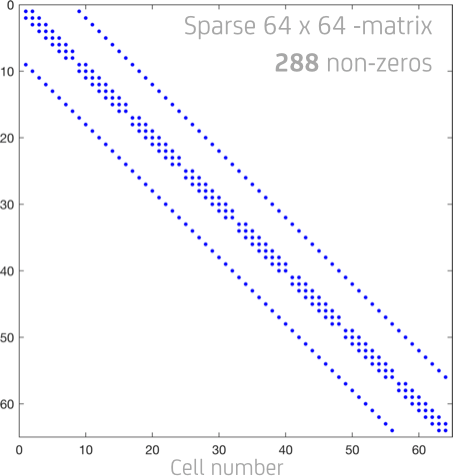
\includegraphics[width=0.85\textwidth]{\figPath/structured_spy.png}
\end{minipage}
\hspace{5mm}
\begin{minipage}[b]{0.475\textwidth}
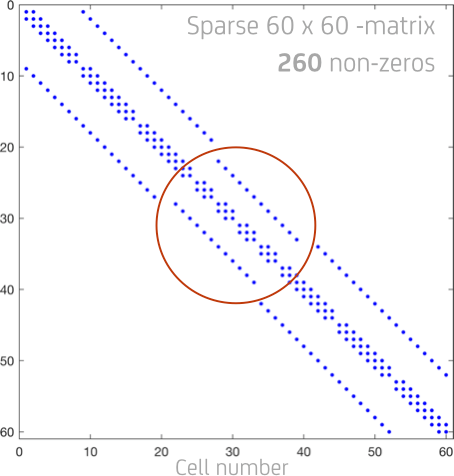
\includegraphics[width=0.85\textwidth]{\figPath/unstructured_spy_zoom.png}
\end{minipage}
\end{center}
\caption[Structured versus unstructured sparsity pattern]{Sparsity patterns of the Poisson matrices for structured and unstructured discretizations:\\
(Left) The structured discretization shows a constantly repeating pattern leading to a highly structured matrix with 288 non-zero entries in total. \\
(Right) The unstructured discretization shows irregularities related to the internal obstruction leading to an irregularly structured matrix with 260 non-zero elements in total.}
\label{FIG_structured_vs_unstructured_spy}
\end{figure}


\newpage


% ------------------------------------------------------------------------------------------------------------------------------------------------------
% Treatment of boundary conditions
% ------------------------------------------------------------------------------------------------------------------------------------------------------
\subsection{Treatment of boundary conditions}
\label{SEC_SCARC_boundary_conditions}

The appropriate treatment of the boundary conditions is of major importance for the accuracy of the numerical pressure solution. There are two basic classes of boundary conditions which must be specified at mesh faces matching with the exterior borders of the computational domain and will be explained subsequently. 

The incorporation of the boundary conditions into Equation (\ref{EQ_SCARC_single_system}) or (\ref{EQ_SCARC_multi_system}) leads to corresponding changes in the matrices and right hand side vectors of the single systems. In order to exemplarily illustrate these mechanisms for the different types of boundary conditions, the 2D-analogue of Equation (\ref{EQ_SCARC_discrete_poisson}) is considered for simplicity,
\be
\frac{\hp_{i+1,k}-2\hp_{ik}+\hp_{i-1,k}}{\dx^2} +
\frac{\hp_{i,k+1}-2\hp_{ik}+\hp_{i,k-1}}{\dz^2}  = R_{ik}\,,
\label{EQ_SCARC_discrete_poisson_two}
\ee
where $R_{ik}$ represents an abbreviation of the corresponding right hand side in 2D.
Note, that for 2D-applications, the number of cells in $y$-direction is fixed to 1 in FDS. Therefore, only the $i$ and $k$ indices are varied in Equation (\ref{EQ_SCARC_discrete_poisson_two}).

\vspace{0.2cm}
\paragraph{Dirichlet boundary conditions:} 
This type of boundary conditions is
applied to open boundaries, where the fluid motion into or out of the domain is driven by the pressure gradient. In this case a value for $\hp$ itself is specified at corresponding grid cells. 

To illustrate the computation of the related matrix entries, an example of the FDS Technical Reference Guide \cite{McGrattan:2018:TG} is used. There, open boundary conditions along the left domain boundary $x = x_{min}$ are considered based on values $\hp_{\ha,k}$ for all indices $k$ along the $z$-direction.
Using these values, the corresponding ghost cell values $H_{0,k}$ along $x = x_{min}$ can be defined by linear extrapolation
\[
\hp_{0,k} = 2 \hp_{\ha,k} - \hp_{1,k}\,.
\]
Replacing the ghost values for all matrix lines with index $i=1$ in Equation (\ref{EQ_SCARC_discrete_poisson_two}), the updated matrix entries for all different values of $k$ look like
\[
\frac{\hp_{2,k}-3\hp_{1,k}}{\dx^2} +
\frac{\hp_{1,k+1}-2\hp_{1,k}+\hp_{1,k-1}}{\dz^2}   
= R_{1,k} - \frac{2}{\dx^2}\hp_{\ha,k}\,.
\]

\vspace{0.2cm}
\paragraph{Neumann boundary conditions:} 
This type of boundary conditions is applied to internal solid obstructions as well as external faces which are entirely determined by a forced flow or a solid. In this case a value for the normal gradient $\partial \hp/\partial n$ must be specified via a corresponding {\it forced-flow} condition
\be 
  \dod{\hp}{n} = -F_n - \dod{u_n}{t}. 
  \label{EQ_SCARC_noflux}
\ee
% for the handling of internal obstructions.  
$F_n$ denotes the normal component of $\bF$ at vents or solid walls and $\partial u_n/\partial t$
a prescribed rate of change in the normal component  of velocity at a forced vent. In case of non reacting solid material, a {\it homogeneous} Neumann condition is present, i.e.\ the right hand side of Equation (\ref{EQ_SCARC_noflux}) is zero.

\newpage
As an example, a forced flow condition is considered for the lower domain boundary $z=z_{min}$,
\[
\frac{\hp_{i,1}-\hp_{i,0}}{\dz} = B_{i,0}\,, 
\]
according to known values $B_{i,0}$ for all indices $i$.
Using the relation $\hp_{i,0}= \hp_{i,1} - \dz \, B_{i,0}$ for all matrix lines  of Equation (\ref{EQ_SCARC_discrete_poisson_two}) with $k=1$ leads to
\be
\frac{\hp_{i+1,1}-2\hp_{i,1}+\hp_{i-1,1}}{\dx^2} +
\frac{\hp_{i,2}-\hp_{i,1}}{\dz^2} \notag  = R_{i,1} + \frac{1}{\dz}B_{i,0}\,.
%\label{EQ_SCARC_discrete_poisson2D}
\ee


\begin{figure}[ht]
\scalebox{0.90}{
\begin{minipage}[t]{1.0\textwidth}
%\begin{center}
\hspace{-0.8in}
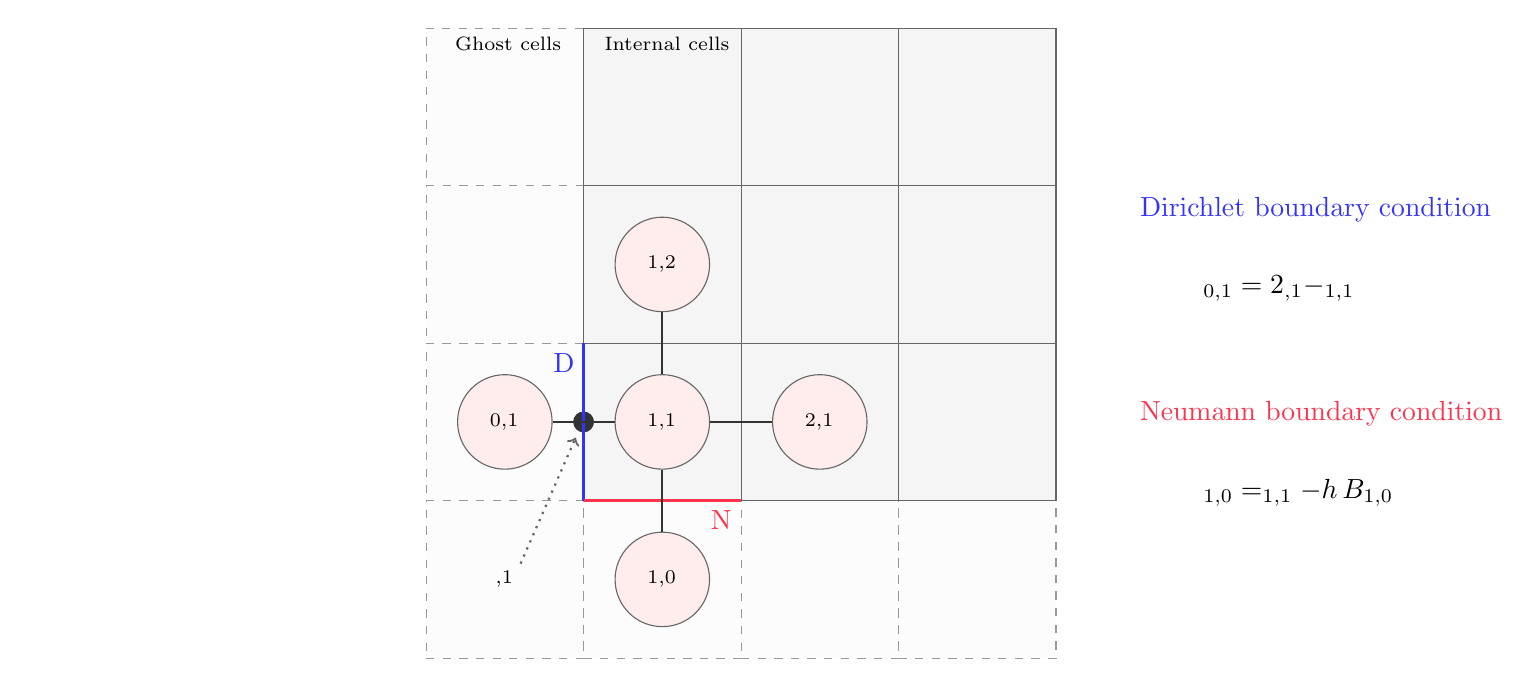
\begin{tikzpicture}[
 inner sep=0.1mm,
 scale=1.0,
 font=\normalsize,
 L4/.style={circle,       draw=black!80, fill=black!80,       thin, minimum size=2.5mm},
 L3/.style={circle,       draw=black!60, fill=red!07,       thin, minimum size=12mm},
 L2/.style={rectangle, draw=black!60, fill=black!04,   thin, minimum size=20mm},
 L1/.style={rectangle, draw=black!40, dashed, fill=black!01,   thin, minimum size=20mm},
 inner sep=0.6mm,
 T1/.style={rectangle, draw=black!02,    thin, minimum size=0.1mm},
 ],
\definecolor{mycolor}{RGB}{255,51,76}
\node (Dummy)   at ( -5, 1)  {};
%
\node [L1]            at ( 1, 1)  {};
\node [L1]            at ( 3, 1)  {};
\node [L1]            at ( 5, 1)  {};
\node [L1]            at ( 7, 1)  {};
%\node [L1]            at ( 9, 1)  {};
\node [L1]            at ( 1, 3)  {};
\node [L1]           at ( 1, 5)  {};
\node [L1]           at ( 1, 7)  {};

\node [L2]            at ( 3, 3)  {};
\node [L2]            at ( 5, 3)  {};
\node [L2]            at ( 7, 3)  {};
%\node [L2]            at ( 9, 3)  {};
%
\node [L2]            at ( 3, 5)  {};
\node [L2]            at ( 5, 5)  {};
\node [L2]            at ( 7, 5)  {};
%
\node [L2]            at ( 3, 7)  {};
\node [L2]            at ( 5, 7)  {};
\node [L2]            at ( 7, 7)  {};

\node [L3]  (HS)   at ( 3, 1)  {$\hp_{1,0}$};
\node [L3]  (HW)  at ( 1, 3)  {$\hp_{0,1}$};
\node [L3]  (HC)   at ( 3, 3)  {$\hp_{1,1}$};
\node [L3]  (HO)  at ( 5, 3)  {$\hp_{2,1}$};
\node [L3]  (HN)  at ( 3, 5)  {$\hp_{1,2}$};

\node [L4]            at ( 2, 3)  {};

%\node                  at ( 2.06, 2.5)  {$\hp_{\,\ha,k}$};
%
%\node [T1]  (DZS)  at ( 3.3,2.0)  {$\dz$};
%\node [T1]  (DZN)  at ( 3.3,4.0)  {$\dz$};
%\node [T1]  (DXW) at ( 2.0,3.3)  {$\dx$};
%\node [T1]  (DXO) at ( 4.0,3.3)  {$\dx$};
%
\draw[->,dotted,thick,black!60] (1.2,1.2) -- (1.9, 2.8);
\node                  at ( 1.0, 1.0)  {$\hp_{\ha,1}$};

\draw [very thick, blue!80]  (2.0,2.0) -- (2.0,4.0);
\draw [very thick, mycolor]  (2.0,2.0) -- (4.0,2.0);

\draw [thick, black!80]  (HC.south) -- (HS.north) ;
\draw [thick, black!80]  (HC.west) -- (HW.east) ;
\draw [thick, black!80]  (HC.north) -- (HN.south) ;
\draw [thick, black!80]  (HC.east) -- (HO.west) ;

\node [anchor=west]   at (0.3, 7.8)  {\scriptsize Ghost cells};
\node [anchor=west]   at (2.2, 7.8)  {\scriptsize Internal cells};
\node [blue!80]    at (1.75, 3.75)  {D};
\node [mycolor]  at (3.75, 1.75)  {N};

\node [anchor=west,blue!80]   at (9, 5.7)  {Dirichlet boundary condition};
\node [anchor=west]   at (9.1, 4.7)  {\qquad $\hp_{0,1} = 2 \hp_{\ha,1} - \hp_{1,1}$};

\node [anchor=west,mycolor]   at (9, 3.1)  {Neumann boundary condition};
\node [anchor=west]   at (9.1, 2.1)  {\qquad $\hp_{1,0}= \hp_{1,1} - h \, B_{1,0}$};

%
\end{tikzpicture}

%\end{center}
\end{minipage}}
\caption{Specification of Dirichlet and Neumann boundary conditions for predefined values for $\hp_{\ha,1}$ and $B_{1,0}$ at the lower left corner of a 2D domain; the ghost cell values $\hp_{0,1}$ and $\hp_{1,0}$ in Equation (\ref{EQ_SCARC_discrete_poisson_two}) are replaced correspondingly.}
\label{FIG_SCARC_bc_setting}
\end{figure}

Suppose that a Dirichlet-boundary meets a Neumann-boundary, as illustrated in Figure~(\ref{FIG_SCARC_bc_setting}) for the lower left corner of a 2D-domain and 
that the grid resolutions in $x$ and $z$-direction are the same, i.e.\ $h=\dx=\dz$, then the matrix line for the grid cell $(1,1)$ finally looks like
\begin{equation*}
\frac{1}{h^2} (\hp_{0,1} - 4\hp_{1,1} + \hp_{1,2} ) = R_{1,1} - 2\frac{1}{h^2} \, \hp_{\ha,1} + \frac{1}{h} \, B_{1,0} \,.
\end{equation*}

The resulting matrix $A$ is irreducibly diagonally dominant which guarantees the solvability by many iterative 
methods.
%
If there is a mix of open and solid surfaces along an external face, the specification of the Dirichlet condition is given precedence to the Neumann condition (i.e.\ it is more important to specify $\hp$ itself than its gradient).
%
In case of multi-mesh applications, it may be necessary to also specify Dirichlet boundary along internal mesh boundaries. However, this depends on the underlying solution technique and will be explained in more detail below.

% ------------------------------------------------------------------------------------------------------------------------------------------------------
% Solution techniques
% ------------------------------------------------------------------------------------------------------------------------------------------------------
\subsection{Parallelization of Poisson solvers}
\label{SEC_SCARC_solver}

Commonly used approaches for the solution of the Poisson equation (\ref{EQ_SCARC_pressure}) 
are either based on direct or iterative solution strategies which will be described in more detail in the next sections of the document. Their efficient parallelization must bridge the gap between the following two very conflicting requirements:
\begin{itemize}
\item {\bf Efficient convergence behavior} ('Globality' preferred)\\
Especially for globally coupled systems such as elliptic equations fast convergence is essentially based on how well an algorithm is able to reproduce global dependencies. Powerful elliptic solvers mainly rest on highly recursive algorithmic structures which strongly couple the overall data of the whole domain. Thus, they have very little inherent parallelism. 
\item {\bf Good parallelization properties} ('Locality' preferred)\\
In contrast to that, methods with a high degree of parallelism often possess a strongly local character. In the ideal case they only need local communication between neighboring subdomains which can nowadays be performed with high computational efficiency on modern parallel platforms.  
\end{itemize}
 
For single-mesh applications the strongly recursive design of traditional elliptic solvers very well reflects the fast and globally acting character of the pressure. In this case, all data required during the computations are easily accessible in the storage of the only processor in use which allows a high computational efficiency. 

For multi-mesh applications the first obvious idea consists in the development of a 1-to-1 parallel analog by splitting up the serial structures according to the new decomposition. But in this case, all required recursive data would be distributed across the entire computing system and would have to be exchanged very frequently which is extremely inefficient from a computational point of view.
In order to increase the degree of parallelism the only remedy is to modify existing techniques or to develop completely new strategies, which are better adapted to modern parallel architectures. However, this process is necessarily associated with a loosening of the global coupling.
New local information can no longer be distributed globally just when it is needed, but only with a time delay or, in order to save computational overhead, only in  reduced or coarser form. Typically, this leads to dependencies on the number of subdomains or the grid resolution associated with losses of numerical efficiency and possible troubles in the correct mapping of actual physical processes. 

These observations can be summarised as follows:
`Well parallelizable algorithms for elliptic problems are often numerically inefficient, numerically efficient algorithms are hardly parallelizable.' The task in designing a suitable solver is therefore to find a suitable compromise. Usually there is no general rule that applies in all cases. Rather, attention must be paid to the specific characteristics of the underlying problem. The optimal strategy for a problem with only a few sub-meshes can be completely different from that for a massively parallel application. For this reason it is of great importance to understand the advantages and disadvantages of different solution strategies and to make the best possible use of this knowledge.


